\documentclass[tikz,border=4pt]{standalone}
\usepackage{amsmath}
\begin{document}
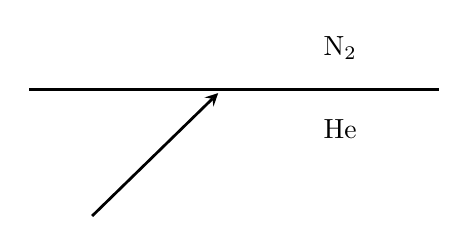
\begin{tikzpicture}[>=stealth, thick, scale=1.0]
  % Thin membrane along y = 0
  \draw[line width=1.1pt] (-2.6, 0) -- (2.6, 0);

  % Gas region labels (chemical formulas)
  \node[above] at (1.35, 0.25) {$\mathrm{N}_2$};
  \node[below] at (1.35, -0.25) {$\mathrm{He}$};

  % Oblique incident sound wave arrow from bottom-left
  \draw[->, line width=1.0pt] (-1.8, -1.6) -- (-0.2, -0.04);
\end{tikzpicture}
\end{document}
